%%=============================================================================
%% Gebruikersonderzoek
%%=============================================================================

\chapter{Gebruikersonderzoek}
\label{ch:gebruikersonderzoek}

\section{Inleiding}

Zoals in Hoofdstuk~\ref{ch:methodologie} werd vermeld zal in dit hoofdstuk een gebruikersonderzoek worden gevoerd op basis van het gebruik van het prototype. Dit onderzoek zal gevoerd worden aan de hand van een enquête bestaande uit drie delen. In het eerste deel zal de demografie van de deelnemers worden onderzocht. In het tweede deel zullen 24 vragen worden gesteld op basis  van de Hexad-schaal om de deelnemers onder te verdelen in verschillende gebruikerstypes. Ten slotte zullen in het derde deel zeven stellingen worden beantwoord om na te gaan of de gebruikersinteractie en -retentie wel degelijk verbeterd is.

\section{Resultaten en analyse}

In de volgende secties zullen de resultaten van de enquête besproken en geanalyseerd worden.

\subsection{Demografie}

\textbf{Resultaat}

De grootte van de steekproef bedroeg 66 deelnemers. De verdeling van deze deelnemers volgens hun geslacht en leeftijden wordt weergegeven in de Tabellen \ref{tab:verdelinggeslacht} en \ref{tab:verdelingleeftijden}. In tabel \ref{tab:verdelinggeslacht} is te zien dat de steekproef uit iets meer vrouwen (57,6\%) dan mannen (42,4\%) bestond. Tabel \ref{tab:verdelingleeftijden} toont dat de deelnemers werden onderverdeeld op basis van hun leeftijd in zeven categorieën. Hieruit is op te maken dat de leeftijden varieerden van jonger dan 18 jaar tot ouder dan 65 jaar. Ook is te zien dat 31,8\% van de bevraagden binnen de leeftijdscategorie 26-35 jaar viel.

\begin{table}
\begin{center}
    \begin{tabular}{c|c|c}
        & \textbf{Totaal} & \textbf{Percentage} (\%) \\
        \hline
        Man & 28 & 42,4\% \\
        \hline
        Vrouw & 38 & 57,6\% \\
    \end{tabular}
\end{center}
\caption{Verdeling van de geslachten.}
\label{tab:verdelinggeslacht}
\end{table}

\begin{table}
    \begin{center}
        \begin{tabular}{c|c|c}
            & \textbf{Totaal} & \textbf{Percentage} (\%) \\
            \hline
            <18 jaar & 4 & 6,1\% \\
            \hline
            18-25 jaar & 12 & 18,2\% \\
            \hline
            26-35 jaar & 21 & 31,8\% \\
            \hline
            36-45 jaar & 7 & 10,6\% \\
            \hline
            46-55 jaar & 5 & 7,6\% \\
            \hline
            56-65 jaar & 11 & 16,7\% \\
            \hline
            >65 jaar & 6 & 9,1\% \\
        \end{tabular}
    \end{center}
\caption{Verdeling van de leeftijden.}
\label{tab:verdelingleeftijden}
\end{table}

\textbf{Bespreking}

De grootte van de steekproef (N = 66) is klein met een ongelijke verdeling van de leeftijdscategorieën. In Tabel \ref{tab:verdelingleeftijden} is te zien dat een aantal van de leeftijdscategorieën een aandeel heeft van minder dan 8 deelnemers. Door deze kleine steekproefgrootte en de ongelijke verdeling van de leeftijden kan deze steekproef niet als representatief worden aanzien.

\subsection{Hexad schaal}

De deelnemers werden onderverdeeld aan de hand van de Gamification User Types Hexad Scale of korter gezegd, de Hexad schaal. Deze onderverdeling gebeurde op basis van de 24 vragen die gesteld werden in het tweede deel van de online enquête. Per gebruikerstype werden vier vragen gesteld op een Likert-schaal van 7 punten. Het totaal van de scores behorende bij deze vier vragen werd opgeteld tot een getal tussen 4 en 28. Zo werd een score bepaald voor elk gebruikerstype. Het maximum van deze scores is het gebruikerstype dat bij die deelnemer past. Per gebruikerstype werd het aantal personen geteld die hierbij de hoogste score behaalde. Soms kwam het voor dat een deelnemer voor meerdere gebruikerstypes een gelijke score behaalde. Als dit voorkwam werd het aantal dat opgeteld werd bij elk gebruikerstype waarvoor de deelnemer een gelijke score heeft berekend door 1 gedeeld door het aantal types. Als een deelnemer bijvoorbeeld een gelijke score heeft behaald bij 3 gebruikerstypes zal bij elk type dan het aantal met 0.33 verhoogd worden.

\textbf{Resultaten}

In figuur \ref{fig:vergelijkingonderzoek} is een vergelijking te zien tussen de verdeling van de steekproef uit het onderzoek van \textcite{Tondello2016} en de verdeling van de steekproef van dit onderzoek. Hierin is te zien dat er een verschil bestaat in de verdeling van de gebruikerstypes. Voor dit onderzoek is een verdeling te zien waarbij Filantropen de grootste groep vormen met 32.0\%, gevolgd door de Socialisers en Presteerders met elk een aandeel van 20.6\%. Daarna komen de Spelers en Vrije geesten met een aandeel van 15.5\% en 11.3\% respectievelijk. Geen enkele van de deelnemers heeft het Ontwrichter gebruikerstype toegewezen gekregen.

\begin{figure}
    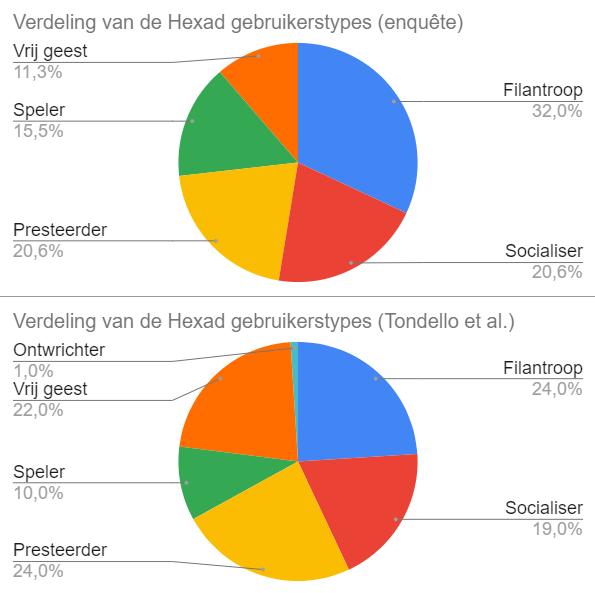
\includegraphics[width=\linewidth]{VergelijkingOnderzoek.png}
    \caption{Vergelijking van de verdeling van de gebruikerstypes.}
    \label{fig:vergelijkingonderzoek}
\end{figure}

De verdeling van de gebruikerstypes per geslacht is te zien in Figuur \ref{fig:verdelinggeslacht}. Hierin is te zien dat een groter aandeel van Filantropen, Socialisers en Presteerders te vinden is bij de vrouwen. Bij de mannen is dan weer een groter aantal Spelers en Vrije geesten te vinden. Via de onafhankelijkheidstoets werd nagegaan of een verband bestaat tussen de gebruikerstypes en het geslacht. In Tabel \ref{tab:onafhankelijkheidstoets} is te zien dat hierbij $\chi^2$(4) = 7.76 werd bekomen en voor p = 0.101 werd bekomen.

\begin{figure}
    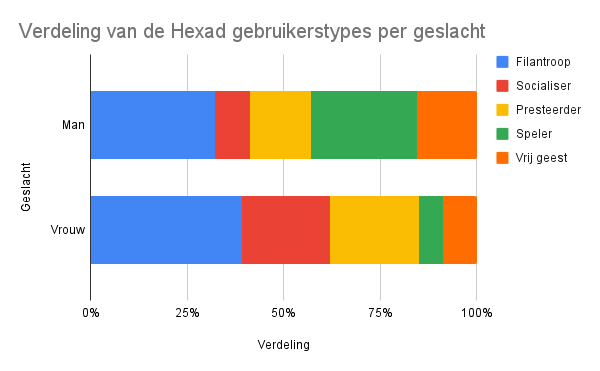
\includegraphics[width=\linewidth]{VerdelingGeslacht.png}
    \caption{Verdeling van de gebruikerstypes per geslacht.}
    \label{fig:verdelinggeslacht}
\end{figure}

\begin{table}
    \begin{center}
    \begin{tabular}{c|c|c|c|c}
        & Onderverdeling & $\chi^2$ & \textit{df} & \textit{p}     \\  
        \hline
        Individueel & Geslacht       & 7.76  & 4  & 0.101 \\
        & Leeftijd       & 18.67 & 24 & 0.770 \\ 
        \hline
        Hybride     & Geslacht       & 12.68 & 5  & 0.027 \\
        & Leeftijd       & 24.28 & 25 & 0.503 \\
    \end{tabular}
    \end{center}
\caption{Resultaten onafhankelijkheidstoets.}
\label{tab:onafhankelijkheidstoets}
\end{table}

In Figuur \ref{fig:verdelingleeftijd} is de verdeling van de gebruikerstypes bij elke leeftijdsgroep te zien. Hieruit blijkt dat hoe ouder een deelnemer is, hoe kleiner de kans is dat hij/zij een Speler is. De kans dat een deelnemer een Filantroop of Socialiser is neemt echter toe met de leeftijd. Met de onafhankelijkheidstoets werd nagegaan of een verband bestaat tussen de gebruikerstypes en de leeftijd. Tabel \ref{tab:onafhankelijkheidstoets} geeft weer dat voor $\chi^2$(24) = 18.67 bekomen werd en voor p = 0.770 bekomen werd.

\begin{figure}
    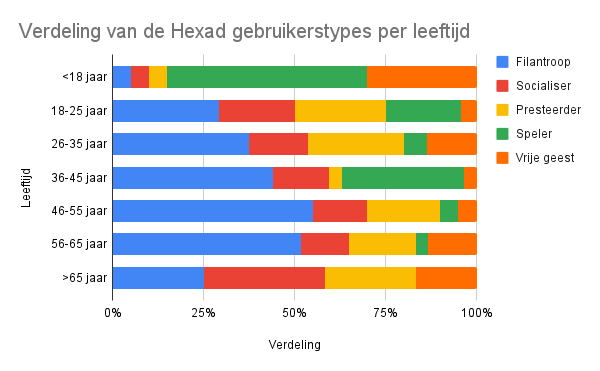
\includegraphics[width=\linewidth]{VerdelingLeeftijd.png}
    \caption{Verdeling van de gebruikerstypes per leeftijd.}
    \label{fig:verdelingleeftijd}
\end{figure}

Zoals eerder al werd vermeld kwam het soms voor dat bij het toewijzen van de gebruikerstypes gelijke scores werden behaald. Van alle deelnemers haalden 18.2\% van hen een gelijke score bij twee gebruikerstypes, 4.5\% haalde een gelijke score bij zowel drie gebruikerstypes als vier gebruikerstypes en 1.5\% haalden een gelijke score bij vijf gebruikerstypes. Geen enkele van de deelnemers haalde een gelijke score bij alle zes de types. Dit wil dus zeggen dat in totaal 28.7\% van de deelnemers geen specifiek gebruikerstype kreeg toegewezen. Het is daarom dat ook werd gekeken naar de verdeling van de zogenaamde hybride gebruikerstypes.

Bij het onderzoek naar de verdeling van de hybride gebruikerstypes werd gekeken naar zowel de gelijke scores als het verschil tussen de twee hoogste scores. Hieruit bleek dat voor 27.3\% van de deelnemers het verschil tussen de hoogste en de tweede hoogste score 1 punt bedraagt, voor 22.7\% bedraagt het verschil 2 punten en voor 10.6\% bedraagt het verschil 3 punten. In combinatie met het aantal gelijke scores wil dit zeggen dat voor 89.3\% van de deelnemers het verschil tussen de hoogste scores ten hoogste 3 punten bedraagt. Dit is een laag verschil en toont aan dat gebruikers niet enkel door hun hoogste score een gebruikerstype kunnen worden toegewezen. In Tabel \ref{tab:aandeelhybridetypes} is daarom het aantal deelnemers te zien bij elke combinatie van toegewezen gebruikerstypes met een maximum verschil in scores van 3.

\begin{table}
    \begin{center}
        \begin{tabular}{c|c|c|c|c|c}
            \multicolumn{5}{c|}{\textbf{Gebruikerstypen}} & \textbf{Percentage} (\%)\\
            \hline
            Filantroop & Socialiser & & & & 16,7\% \\
            \hline
            Filantroop & Presteerder & & & & 16,7\%\\
            \hline
            Filantroop & Vrije geest & & & & 9,1\%\\
            \hline
            Presteerder & Speler & & & & 9,1\%\\
            \hline
            Presteerder & Socialiser & & & & 6,1\%\\
            \hline
            Speler & Vrije geest & & & & 4,5\%\\
            \hline
            Filantroop & Socialiser & Vrije geest & & & 4,5\%\\
            \hline
            Presteerder & Vrije geest & & & & 3,0\%\\
            \hline
            Socialiser & Vrije geest & & & & 3,0\%\\
            \hline
            Filantroop & Presteerder & Socialiser & & & 3,0\%\\
            \hline
            Filantroop & Speler & & & & 1,5\%\\
            \hline
            Filantroop & Socialiser & Speler & & & 1,5\%\\
            \hline
            Filantroop & Presteerder & Vrije geest & & & 1,5\%\\
            \hline
            Filantroop & Presteerder & Speler & & & 1,5\%\\
            \hline
            Presteerder & Speler & Vrije geest & & & 1,5\%\\
            \hline
            Filantroop & Socialiser & Speler & Vrije geest & & 1,5\%\\
            \hline
            Presteerder & Socialiser & Speler & Vrije geest & & 1,5\%\\
            \hline
            Filantroop & Presteerder & Socialiser & Vrije geest & & 1,5\%\\
            \hline
            Filantroop & Presteerder & Speler & Socialiser & Vrije geest & 1,5\%\\
        \end{tabular}
    \end{center}
    \caption{Aandeel van de hybride gebruikerstypes.}
    \label{tab:aandeelhybridetypes}
\end{table}

Figuur \ref{fig:hybridegeslacht} toont de verdeling van de zes meeste voorkomende hybride gebruikerstypes per geslacht. Bij de vrouwen is te zien dat ze bestaan uit een groter aandeel Filantroop-Presteerders en Filantroop-Socialisers. Bij de mannen zijn dan weer meer Presteerder-Spelers en Speler-Vrije geesten te vinden. Het Filantroop-Presteerder hybride gebruikerstype is bij de mannen niet te vinden. Met de onafhankelijkheidstoets werd nagegaan of een verband bestaat tussen de hybride gebruikerstypes en het geslacht. In Tabel \ref{tab:onafhankelijkheidstoets} is te zien dat voor $\chi^2$(5) = 12.68 bekomen werd en voor p = 0.027 bekomen werd.

\begin{figure}
    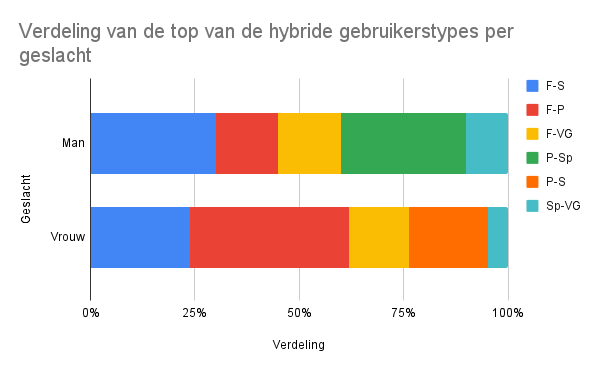
\includegraphics[width=\linewidth]{HybrideGeslacht.png}
    \caption{Verdeling van de top van de hybride gebruikerstypes per geslacht.}
    \label{fig:hybridegeslacht}
\end{figure}

In Figuur \ref{fig:hybrideleeftijd} is te zien dat het aandeel van de Filantroop-Socialisers en Filantroop-Presteerders met de leeftijd stijgt. Presteerder-Spelers en Speler-Vrije geesten zijn dan weer niet te vinden bij de oudere deelnemers. Aan de hand van de onafhankelijkheidstoets werd nagegaan of een verband bestaat tussen de hybride gebruikerstypes en de leeftijd. Tabel \ref{tab:onafhankelijkheidstoets} toont dat voor $\chi^2$(25) = 24.28 bekomen werd en voor p = 0.503 bekomen werd.

\begin{figure}
    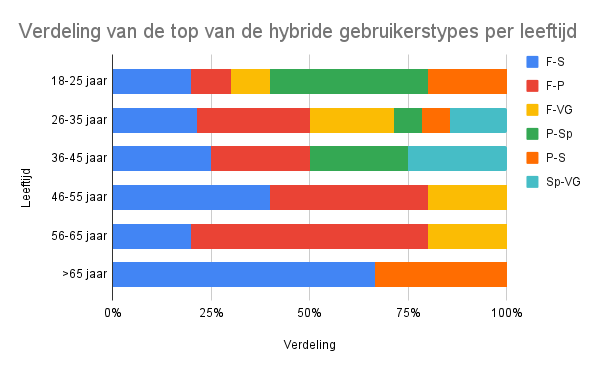
\includegraphics[width=\linewidth]{HybrideLeeftijd.png}
    \caption{Verdeling van de top van de hybride gebruikerstypes per leeftijd.}
    \label{fig:hybrideleeftijd}
\end{figure}

\textbf{Bespreking}

Figuur \ref{fig:vergelijkingonderzoek} toont een vergelijking tussen de verdeling van de steekproef uit het onderzoek van \textcite{Tondello2016} en de verdeling van de steekproef van dit onderzoek. Hierin is te zien dat er een verschil bestaat in de verdeling van de gebruikerstypes. In het onderzoek van \textcite{Tondello2016} zijn de Filantropen (24.0\%), de Presteerders (24.0\%) en de Vrij geesten (22.0\%) de dominante types terwijl in dit onderzoek de Filantropen (32.0\%), de Socialisers (20.6\%) en de Presteerders (20.6\%) het grootste aandeel vormen. Het grootste verschil met hun onderzoek is dat de Vrije geesten (11.3\%) maar een half zo groot aandeel vormen binnen dit onderzoek. Het Ontwrichter gebruikerstype ontbreekt aangezien geen enkele deelnemer dit type toegewezen gekregen heeft. Dit is vergelijkbaar met het onderzoek van Tondello et al. waar slechts 1.0\% als Ontwrichter gezien werd.

Uit de resultaten van de onafhankelijkheidstoets, te zien in Tabel \ref{tab:onafhankelijkheidstoets}, kan afgeleid worden dat tussen de individuele gebruikerstypes en het geslacht geen significante associatie bestaat. Ook tussen de individuele gebruikerstypes en de leeftijd kan geen significante associatie worden opgemaakt. Voor de hybride gebruikerstypes valt op dat de resultaten aangeven dat een associatie met het geslacht bestaat. Tussen de hybride gebruikerstypes en de leeftijd tonen de resultaten opnieuw dat geen associatie hiertussen bestaat. Deze resultaten kunnen echter als onbetrouwbaar worden beschouwd gezien de kleine steekproefgrootte en gelet op het feit dat niet aan de regel van Cochran is voldaan.

\subsection{Prototype}

Nadat de deelnemers alle vragen hadden beantwoord uit het tweede deel van de enquête om hen te gaan onderverdelen in verschillende gebruikerstypes, werden aan hen zeven stellingen voorgelegd. Zoals in Hoofdstuk~\ref{ch:methodologie} werd vermeld, zijn deze stellingen gebaseerd op de ervaring bij het gebruiken van het prototype. De eerste vier stellingen waren van toepassing op het puntensysteem en de overige stellingen waren respectievelijk van toepassing op het scorebord, het badgesysteem en de beloningswinkel. De deelnemers gaven bij deze stellingen aan of ze hiermee akkoord gingen of niet. Dit gebeurde aan de hand van een Likert-schaal van 5 punten (1 = helemaal niet akkoord, 2 = niet akkoord, 3 = neutraal, 4 = akkoord, 5 = volledig akkoord). Hieronder volgt een opsomming van de verschillende stellingen:

\begin{itemize}
    \item Stelling 1 (S1): \textit{Ik ben nu sneller bereid om meer enquêtes in te vullen.}
    \item Stelling 2 (S2): \textit{Ik wil meer enquêtes invullen om mijn aantal behaalde punten te verhogen.}
    \item Stelling 3 (S3): \textit{Ik ben nu sneller bereid om enquêtes tot het einde in te vullen omdat ik voor elke ingevulde pagina punten krijg.}
    \item Stelling 4 (S3): \textit{Ik wil meer enquêtes delen om mijn aantal behaalde punten te verhogen.}
    \item Stelling 5 (S5): \textit{Ik wil meer enquêtes invullen om mijn rangschikking op het leaderboard (scorebord) te verhogen.}
    \item Stelling 6 (S6): \textit{Ik wil meer enquêtes invullen om extra badges te behalen.}
    \item Stelling 7 (S7): \textit{Ik wil meer enquêtes invullen om beloningen te kunnen kopen in de rewardshop (beloningswinkel).}
\end{itemize}

\textbf{Resultaten}

Om te gaan bepalen of de gebruikersinteractie en -retentie wel degelijk verbeterd is, werd voor de individuele gebruikerstypes nagegaan wat hun respectievelijke scores waren bij de verschillende stellingen. Voor de hybride gebruikerstypes werd ook nagegaan wat hun scores waren maar hier werd de analyse beperkt tot de vier grootste groepen van de hybride gebruikerstypes. De overige groepen hadden slechts een grootte van 3 of kleiner. In dit deel van het onderzoek werd gekozen om de scores niet verder onder te verdelen tussen geslacht of leeftijd. Deze beslissing werd genomen op basis van de resultaten van de onafhankelijkheidstoets uit het vorige deel, waar aangetoond werd dat geen significante associatie bestaat tussen de gebruikerstypes en het geslacht of de leeftijd.

De Figuren gaande van \ref{fig:s1} tot \ref{fig:s7_hybride} geven de resultaten weer per stelling. Tabel \ref{tab:mediaan} geeft de mediaan van de scores weer per gebruikerstype en per stelling.

\begin{table}
    \begin{center}
    \begin{tabular}{c|c|c|c|c|c|c|c|c}
        & Gebruikerstypes & S1 & S2 & S3  & S4  & S5  & S6 & S7  \\
        \hline
        Individueel & Filantroop             & 3  & 3  & 3   & 2   & 2   & 2  & 3   \\
        & Socialiser             & 3  & 3  & 3   & 3   & 2.5 & 3  & 4   \\
        & Vrije geest            & 3  & 3  & 3   & 2.5 & 2   & 2  & 4   \\
        & Presteerder            & 3  & 4  & 4   & 3   & 3   & 3  & 4   \\
        & Speler                 & 4  & 4  & 4   & 4   & 4   & 3  & 5   \\
        \hline
        Hybride     & Filantroop-Presteerder & 1  & 1  & 1   & 1   & 1   & 1  & 1   \\
        & Filantroop-Socialiser  & 3  & 3  & 3   & 2   & 2   & 2  & 3   \\
        & Filantroop-Vrije geest & 3  & 3  & 3   & 2.5 & 2   & 2  & 3.5 \\
        & Presteerder-Speler     & 4  & 5  & 4.5 & 4   & 4   & 4  & 5  
    \end{tabular}
    \end{center}
\caption{Mediaan van de scores bij elke stelling.}
\label{tab:mediaan}
\end{table}

\textbf{Stelling 1}

In Figuur \ref{fig:s1} is de verdeling van de scores voor de individuele gebruikerstypes van de eerste stelling te zien.  Bij deze stelling werd onderzocht of gebruikers nu meer bereid zijn om enquêtes te gaan invullen na de toevoeging van de game-design elementen aan het prototype In de figuur is te zien dat bijna 50\% van de Presteerders en meer dan 75\% van de Spelers na het gebruik van het prototype bereid zijn om meer enquêtes in te vullen.

\begin{figure}
    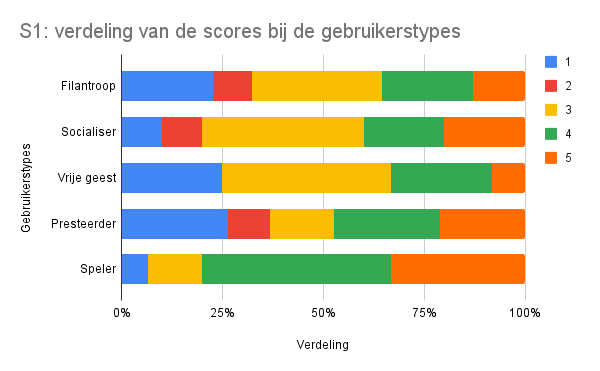
\includegraphics[width=\linewidth]{S1.png}
    \caption{Verdeling van de scores bij de individuele gebruikerstypes voor stelling 1.}
    \label{fig:s1}
\end{figure}

Figuur \ref{fig:s1_hybride} geeft de verdeling van de scores voor de hybride gebruikerstypes van de eerste stelling weer. Daarop is te zien dat geen enkele van de Presteerder-Spelers een score lager dan 4 aangaven, wat wil zeggen dat ze akkoord of volledig akkoord gingen met deze stelling. De meerderheid van de Filantroop-Presteerders gaf dan weer aan dat ze helemaal niet akkoord waren met deze stelling.

\begin{figure}
    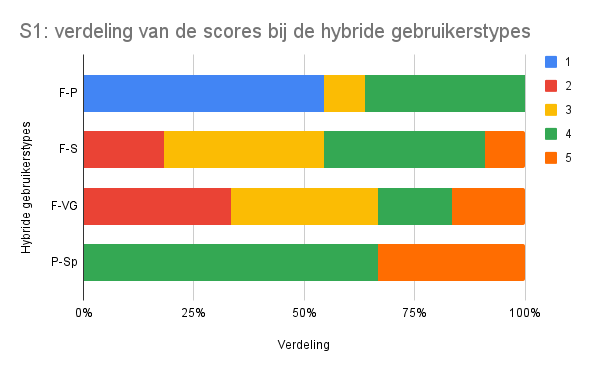
\includegraphics[width=\linewidth]{S1_Hybride.png}
    \caption{Verdeling van de scores bij de hybride gebruikerstypes voor stelling 1.}
    \label{fig:s1_hybride}
\end{figure}

Tabel \ref{tab:mediaan} geeft de mediaan van de scores weer. Daarop is te zien dat de scores van de Spelers en de Presteerder-Spelers een mediaan hebben van 4, wat wil zeggen dat de meerderheid van hen akkoord ging met deze stelling. De mediaan van de scores van de Filantroop-Presteerders toont dan weer dat het grootste deel van hen niet akkoord ging met deze stelling.

\textbf{Stelling 2}

De verdeling van de scores voor de individuele gebruikerstypes van de tweede stelling wordt weergegeven in Figuur \ref{fig:s2}. Hier werd onderzocht of de deelnemers na het gebruik van het prototype meer bereid zijn om enquêtes in te vullen om hun aantal verzamelde punten te verhogen. Meer dan 50\% van zowel de Presteerders als de Spelers gaven een hoge score aan wat wil zeggen dat ze met deze stelling akkoord of volledig akkoord gingen.

\begin{figure}
    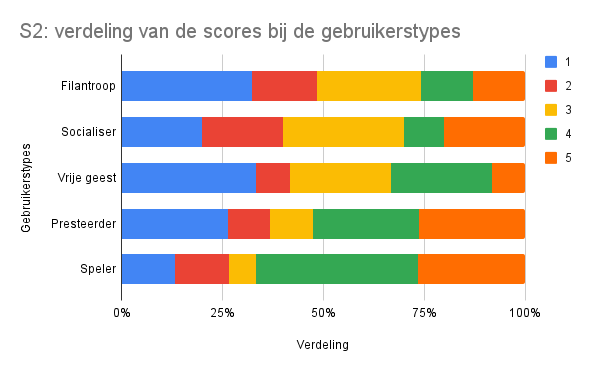
\includegraphics[width=\linewidth]{S2.png}
    \caption{Verdeling van de scores bij de individuele gebruikerstypes voor stelling 2.}
    \label{fig:s2}
\end{figure}

Voor de verdeling van de scores voor de hybride gebruikerstypes van de tweede stelling is te zien in Figuur \ref{fig:s2_hybride} dat de Presteerder-Spelers opnieuw akkoord of volledig akkoord gingen. Van alle Filantroop-Presteerders gaf de meerderheid weer aan dat ze niet akkoord gingen.

\begin{figure}
    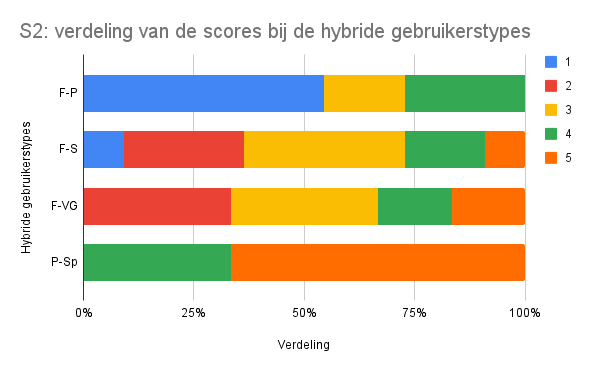
\includegraphics[width=\linewidth]{S2_Hybride.png}
    \caption{Verdeling van de scores bij de hybride gebruikerstypes voor stelling 2.}
    \label{fig:s2_hybride}
\end{figure}

De mediaan van de scores, te zien in tabel \ref{tab:mediaan}, toont dat het grootste deel van de Presteerders en de Spelers akkoord ging met deze stelling. De mediaan van 5 bij de Presteerder-Spelers geeft weer dat de meeste van hen volledig akkoord gingen. Ook is opnieuw een mediaan van 1 te zien bij de Filantroop-Presteerders, wat wil zeggen dat het merendeel helemaal niet akkoord ging met deze stelling.

\textbf{Stelling 3}

Bij de derde stelling werd onderzocht of de deelnemers meer bereid zijn om enquêtes in te vullen omdat ze bij elke ingevulde pagina punten toegewezen krijgen. Figuur \ref{fig:s3} toont aan dat bijna 75\% van de Spelers hiermee akkoord gingen. Ook gaf meer dan 50\% van de Presteerders aan dat ze met deze stelling akkoord waren. Bijna de helft van de Filantropen was echter niet akkoord met deze stelling.

\begin{figure}
    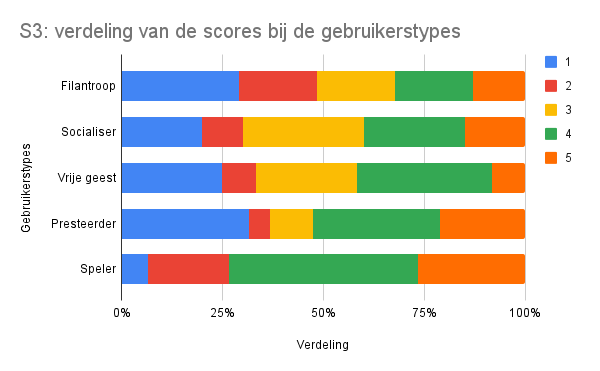
\includegraphics[width=\linewidth]{S3.png}
    \caption{Verdeling van de scores bij de individuele gebruikerstypes voor stelling 3.}
    \label{fig:s3}
\end{figure}

De scores van de hybride gebruikerstypes zijn te zien in Figuur \ref{fig:s3_hybride}. Net zoals bij de vorige stelling gaf geen enkele van de Presteerder-Spelers een score lager dan 4 aan. Ook gaf meer dan 50\% van de Filantroop-Presteerders opnieuw aan dat ze niet akkoord zijn met deze stelling.

\begin{figure}
    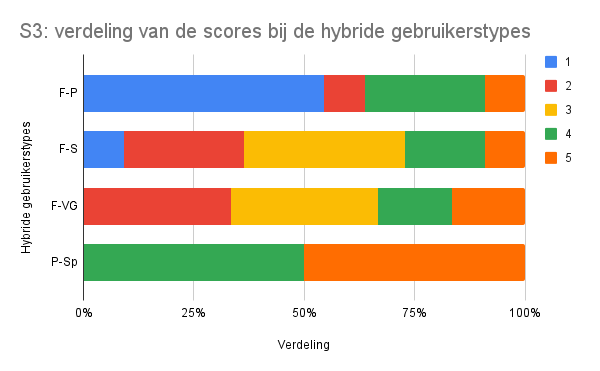
\includegraphics[width=\linewidth]{S3_Hybride.png}
    \caption{Verdeling van de scores bij de hybride gebruikerstypes voor stelling 3.}
    \label{fig:s3_hybride}
\end{figure}

Tabel \ref{tab:mediaan} toont opnieuw aan dat de meerderheid van de Presteerders, de Spelers en de Presteerder-Spelers akkoord ging met deze stelling, af te leiden uit de mediaan van 4 en 4.5. Voor de Filantroop-Presteerders zet dezelfde trend zich voort, waarbij een mediaan te zien is van 1. Dit wil dus zeggen dat ze opnieuw voor het grootste deel helemaal niet akkoord gingen met de stelling.

\textbf{Stelling 4}

In Figuur \ref{fig:s4} zijn de scores van de individuele gebruikerstypes voor stelling 4 te zien. Hierbij werd onderzocht of de deelnemers meer bereid zijn om enquêtes te gaan delen om punten te verzamelen. Uit de figuur is opnieuw op te maken dat meer dan 50\% van de Spelers aangaven dat ze met deze stelling akkoord gingen. Bij de verdeling van de scores van de Presteerders is een lichte daling te merken in vergelijking met de vorige stelling waardoor het aantal dat met deze stelling akkoord ging daalt tot net iets onder 50\%.

\begin{figure}
    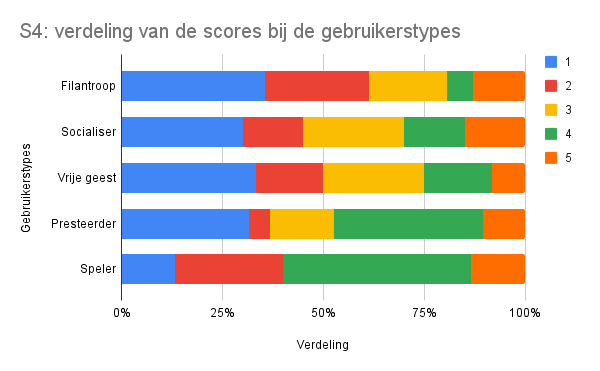
\includegraphics[width=\linewidth]{S4.png}
    \caption{Verdeling van de scores bij de individuele gebruikerstypes voor stelling 4.}
    \label{fig:s4}
\end{figure}

Figuur \ref{fig:s4_hybride} toont de scores bij stelling 4 voor de hybride gebruikerstypes. Hierbij valt sterk op dat alle Presteerder-Spelers een score van 4 aangaven wat wil zeggen dat ze akkoord gingen met de stelling maar niet volledig. Voor de overige hybride gebruikerstypes gaf 50\% of meer aan dat ze niet akkoord gingen met deze stelling.

\begin{figure}
    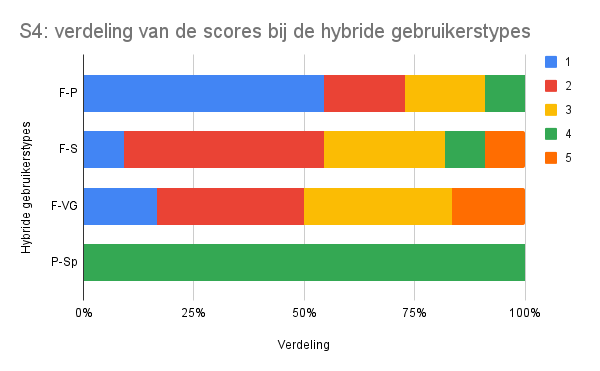
\includegraphics[width=\linewidth]{S4_Hybride.png}
    \caption{Verdeling van de scores bij de hybride gebruikerstypes voor stelling 4.}
    \label{fig:s4_hybride}
\end{figure}

De mediaan van de scores (Tabel \ref{tab:mediaan}) voor de Spelers en Presteerder-Spelers bedraagt 4, wat voor de Presteerder-Spelers een lichte daling is. Echter blijven ze nog steeds grotendeels akkoord met deze stelling, net zoals de Spelers. Voor de Filantropen, de Vrije geesten, de Presteerders, de Filantroop-Presteerders, de Filantroop-Socialisers en de Filantroop-Vrije geesten is ook een daling merkbaar. Dit wil zeggen dat, in vergelijking met de vorige stelling, een groter deel niet akkoord is met deze stelling. Voor de Filantroop-Presteerders blijft, net zoals alle vorige stellingen, een mediaan van 1 behouden.

\textbf{Stelling 5}

Stelling 5 onderzocht of de deelnemers bereid zijn om meer enquêtes in te vullen om hun rangschikking op het scorebord te verhogen. In Figuur \ref{fig:s5} is te zien dat meer dan 50\% van de Spelers en net geen 50\% van de Presteerders aangaven dat ze met deze stelling akkoord gingen. Bij de Socialisers gaf 50\% aan dat ze niet met deze stelling akkoord gingen net zoals de meerderheid van de Filantropen en de Vrije geesten.

\begin{figure}
    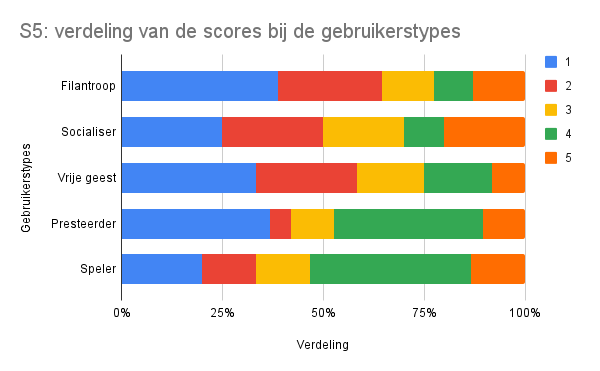
\includegraphics[width=\linewidth]{S5.png}
    \caption{Verdeling van de scores bij de individuele gebruikerstypes voor stelling 5.}
    \label{fig:s5}
\end{figure}

Figuur \ref{fig:s5_hybride} geeft voor de hybride gebruikerstypes weer dat, in tegenstelling tot de vorige stellingen, niet alle Presteerder-Spelers akkoord gingen met deze stelling. Bij de Filantroop-Socialisers en Filantroop-Vrij geesten gaf meer dan 50\% aan dat ze niet akkoord gingen met de stelling. Bijna alle Filantroop-Presteerders gingen niet akkoord met de stelling.

\begin{figure}
    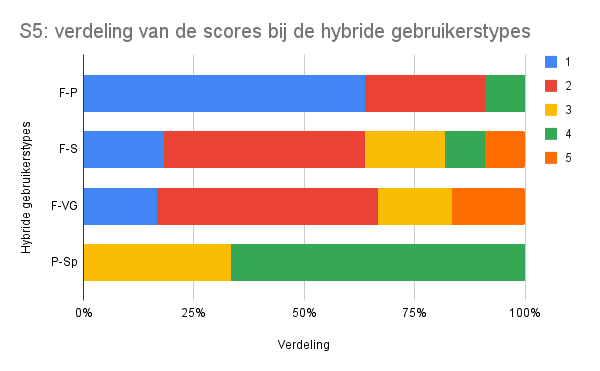
\includegraphics[width=\linewidth]{S5_Hybride.png}
    \caption{Verdeling van de scores bij de hybride gebruikerstypes voor stelling 5.}
    \label{fig:s5_hybride}
\end{figure}

In Tabel \ref{tab:mediaan} is een mediaan van 4 voor zowel de Spelers als de Presteerder-Spelers te zien, waardoor opnieuw kan afgeleid worden dat de meerderheid van hen akkoord gaat met deze stelling. Voor de Filantropen, Socialisers, Vrije geesten en de overige hybride gebruikerstypes is een mediaan te zien van 2.5 of lager. Dit wil zeggen dat de helft of meer van hen niet akkoord ging met de vijfde stelling.

\textbf{Stelling 6}

Om de invloed van de badges binnen het prototype te onderzoeken werd aan de deelnemers gevraagd of ze bereid zijn meer enquêtes in te vullen om badges te behalen. Figuur \ref{fig:s6} toont aan dat voor de eerste maal minder dan 50\% van de Spelers met deze stelling akkoord ging. De meerderheid van de Filantropen en Vrije geesten ging niet akkoord met deze stelling.

\begin{figure}
    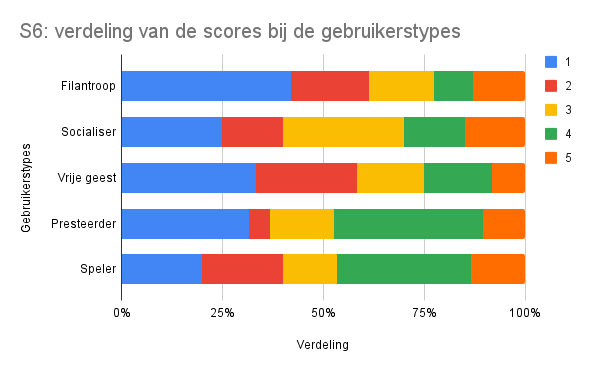
\includegraphics[width=\linewidth]{S6.png}
    \caption{Verdeling van de scores bij de individuele gebruikerstypes voor stelling 6.}
    \label{fig:s6}
\end{figure}

Bij de hybride gebruikerstypes, waarvan de score te zien is in Figuur \ref{fig:s6_hybride}, is dezelfde verdeling van de scores te zien voor de Presteerder-Spelers als bij de vorige stelling. Daaruit is af te leiden dat opnieuw niet alle Presteerder-Spelers akkoord gingen met deze stelling. Ook gaf meer dan 50\% van de Filantroop-Socialisers en de Filantroop-Vrije geesten opnieuw aan dat ze niet akkoord gingen met deze stelling. Voor de Filantroop-Presteerders is het aantal dat niet akkoord ging met de stelling iets gedaald in vergelijking met de vorige stelling maar nog steeds hoger dan 50\%.

\begin{figure}
    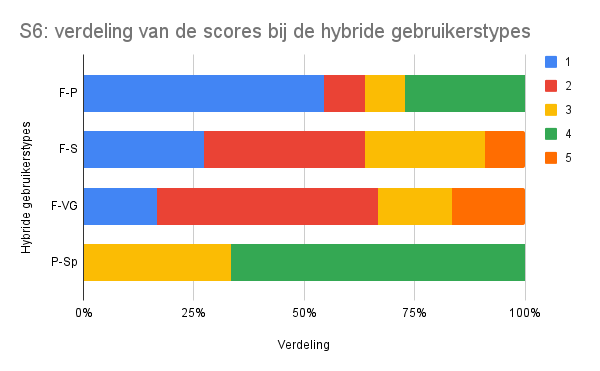
\includegraphics[width=\linewidth]{S6_Hybride.png}
    \caption{Verdeling van de scores bij de hybride gebruikerstypes voor stelling 6.}
    \label{fig:s6_hybride}
\end{figure}

Tabel \ref{tab:mediaan} toont dat voor de Spelers de mediaan van hun scores voor de eerste en enige maal lager dan 4 is, wat erop wijst dat minder dan de helft akkoord ging met deze stelling. De Presteerder-Spelers blijven een mediaan behouden van 4 wat erop wijst dat de meerderheid akkoord ging. Voor de overige gebruikerstypes blijft dezelfde mediaan behouden in vergelijking met de vorige stelling maar met één uitzondering, de Socialisers. Bij hen is de mediaan met een half punt gestegen wat wil zeggen dat het deel dat niet akkoord ging gedaald is.

\textbf{Stelling 7}

Bij de zevende en laatste stelling werd de invloed van de beloningswinkel onderzocht. Aan de deelnemers werd gevraagd of ze meer bereid zijn om enquêtes in te vullen om beloningen te kunnen aanschaffen. In Figuur \ref{fig:s7} is te zien dat de deelnemers over het algemeen het meeste akkoord waren met deze stelling. Meer dan 50\% van de Socialisers, Vrije geesten, Presteerders en Spelers gaf aan dat ze met deze stelling akkoord gingen. Enkel bij de Filantropen was het aantal lager dan 50\%.

\begin{figure}
    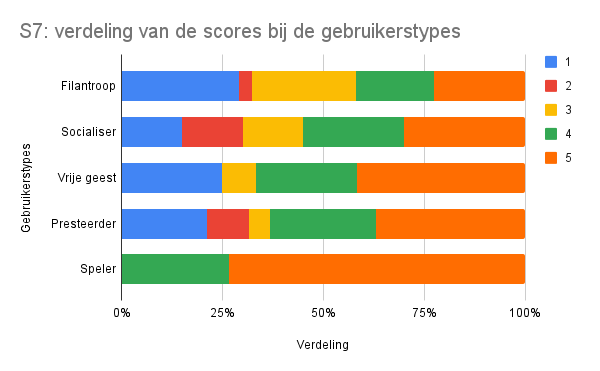
\includegraphics[width=\linewidth]{S7.png}
    \caption{Verdeling van de scores bij de individuele gebruikerstypes voor stelling 7.}
    \label{fig:s7}
\end{figure}

Figuur \ref{fig:s7_hybride} geeft weer dat bij de scores van de hybride gebruikerstypes de Presteerder-Spelers allemaal akkoord gingen met de stelling, meer dan 75\% was zelfs volledig akkoord. Voor de Filantroop-Vrije geesten was 50\% akkoord. De meerderheid van de Filantroop-Presteerders ging niet akkoord met de stelling.

\begin{figure}
    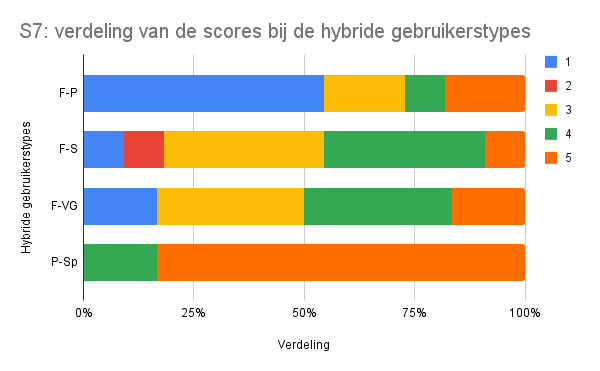
\includegraphics[width=\linewidth]{S7_Hybride.png}
    \caption{Verdeling van de scores bij de hybride gebruikerstypes voor stelling 7.}
    \label{fig:s7_hybride}
\end{figure}

Tabel \ref{tab:mediaan} toont aan dat de mediaan voor bijna alle gebruikerstypes de hoogste waarde heeft, met zelfs een mediaan van 5 voor zowel de Spelers als de Presteerder-Spelers. Dit wil zeggen dat voor bijna alle types het grootste deel akkoord ging met de laatste stelling. Enkel bij de Filantropen, de Filantroop-Presteerders en de Filantroop-Socialisers blijft het aandeel dat akkoord ging kleiner dan de helft. Voor de Filantroop-Presteerders is geen verandering merkbaar met vorige stellingen. De mediaan van 1 blijft behouden wat opnieuw wil zeggen dat het grootste deel niet akkoord ging met deze stelling.

\textbf{Bespreking}

Zoals eerder werd vermeld waren de eerste vier stellingen van toepassing op het puntensysteem. Hierbij werd verwacht dat vooral de Spelers door dit systeem gemotiveerd zouden worden. Uit de resultaten voor deze stellingen is te zien dat meer dan 50\% van de Spelers en alle Presteerder-Spelers akkoord gingen met deze stellingen, wat de verwachting bevestigd. Bij de vierde stelling is echter wel te merken dat, in vergelijking met de vorige stellingen, een groter aantal Spelers niet akkoord ging en geen enkele Presteerder-Spelers volledig akkoord gingen. Een verklaring hiervoor is dat bij de eerste drie stellingen de testenquête op het prototype slechts eenmaal moest voltooid worden om de punten te verzamelen. Voor de vierde stelling moest de testenquête gedeeld worden om punten te verkrijgen. Dit vereiste echter enige samenwerking tussen de deelnemers en dat de testenquête meerdere malen moest voltooid worden. De relatief lagere scores voor de vierde stelling kunnen dus verklaard worden door het extra werk dat moest uitgevoerd worden.

Bij de vijfde stelling werd verwacht dat vooral de Spelers en Presteerders gemotiveerd zouden worden door het gebruik van een scorebord. De resultaten van de individuele gebruikerstypes ondersteunen deze verwachting. Bij de hybride gebruikerstypes is echter een verschillend resultaat te zien.  De Presteerder-Spelers gingen bij deze stelling voor de eerste maal niet allemaal akkoord. Bij de Filantroop-Presteerders werd verwacht dat door de combinatie met het Presteerder gebruikerstype het aantal dat akkoord ging hoger zou zijn. Uit de resultaten is echter op te maken dat bijna alle Filantroop-Presteerders niet akkoord gingen met deze stelling.

Voor de zesde stelling werd verwacht dat vooral de Spelers gemotiveerd zouden worden door het verkrijgen van badges. De resultaten tonen echter dat voor de eerste en enige keer minder dan 50\% van de Spelers akkoord gingen en dat opnieuw niet alle Presteerder-Spelers akkoord gingen. Dit kan verklaard worden door technische problemen met het weergeven van de badge. Als noodoplossing werd gekozen om een afbeelding te nemen van het verkrijgen van een badge en dit voor te leggen aan de deelnemers. Dit bereikte echter niet het gewenste psychologische effect van het verdienen van een badge waardoor de resultaten lager zijn dan verwacht voor de Spelers.

Bij de laatste stelling werd verwacht dat de Spelers het meeste gemotiveerd zouden worden door de beloningen. De resultaten bevestigen dit vermoeden en tonen aan dat alle Spelers en Presteerder-Spelers met deze stelling akkoord gingen. Ook is te merken dat bij de overige gebruikerstypes het grootste aantal van hen akkoord ging in vergelijking met alle andere stellingen. Een verklaring kan hiervoor gegeven worden doordat deelnemers een fysieke beloning kunnen verkrijgen voor hun prestaties.

De resultaten van alle stellingen tonen aan dat bij de individuele en de hybride gebruikerstypes meer dan 50\% van de Presteerder-Spelers met alle stellingen akkoord of zelfs volledig akkoord gingen. Voor de Spelers is hetzelfde resultaat te zien met uitzondering van de zesde stelling. Aan de hand van deze resultaten valt dus af te leiden dat Spelers en Presteerder-Spelers vooral door punten, badges en scoreborden worden gemotiveerd. Uit de onderzoeken van zowel \textcite{Tondello2016} als \textcite{Carreno2018} blijkt dat Spelers het sterkst gemotiveerd worden door extrinsieke beloningen, waardoor dat de ontwerpelementen die het beste passen bij Spelers punten, scoreborden en badges zijn. Deze resultaten werden opnieuw bevestigd binnen dit onderzoek.
    
Bij de resultaten van de individuele en hybride gebruikerstypes valt ook op dat verschillende resultaten worden bekomen. Dit toont aan de gebruikers niet enkel door hun hoogste score bij de gebruikerstypes kunnen worden geïdentificeerd maar dat ook het ook nodig is om de overige scores te onderzoeken aangezien deze dicht bij elkaar liggen. 

Uit al deze resultaten blijkt dat een gebruikersonderzoek nodig is om te kunnen bepalen welke ontwerpelementen geïmplementeerd moeten worden en op welke manier ze moeten aangepast worden. Als bijvoorbeeld blijkt uit dit onderzoek dat de gebruikers vooral bestaan uit Presteerder-Spelers is het logischer dat de focus vooral wordt gelegd op scoreborden en puntensystemen. Echter als vooral Socialiser-Vrij geesten voorkomen dan zou het toevoegen van verkenningstaken met een sociaal aspect een meerwaarde zijn.



